%% ----------------------------------------------------------------------
%% START OF FILE
%% ----------------------------------------------------------------------
%% 
%% Filename: ch02-options.tex
%% Author: Fred Qi
%% Created: 2012-12-26 09:15:56(+0800)
%% 
%% ----------------------------------------------------------------------
%%% CHANGE LOG
%% ----------------------------------------------------------------------
%% Last-Updated: 2015-05-14 20:48:32(+0300) [by Fred Qi]
%%     Update #: 77
%% ----------------------------------------------------------------------
\ifx\allfiles\undefined
\documentclass[bachelor,print,msfonts]{xduthesis}

% 这里是可能用到的其他宏包,根据自己论文撰写的需要添加
\usepackage{listings}
\usepackage{overpic}
\lstset{language=TeX, basicstyle=\ttfamily}

\newcommand{\figref}[1]{图\ref{#1}}
\newcommand{\sArt}{state-of-the-art}
\newcommand{\wyh}[1]{{\textcolor{blue}{#1}}}
\newcommand{\secref}[1]{Sec. \ref{#1}}
\newcommand{\tabref}[1]{Tab.~\ref{#1}}
\newcommand{\thudot}[1]{} % thubib.bst 定义每条参考文献最后的点\thudot
\graphicspath{{./}{./img/}{./fig/}{./image/}{./figure/}{./picture/}}
\newcommand{\bs}{\boldsymbol}
\usepackage{float}
\setcounter{chapter}{1}

\begin{document}
\mainmatter
\fi

\chapter{Trisoup顶点标识与位置信息的熵编码优化}
\label{cha:options}
Trisoup几何信息编码算法中对顶点标识信息和位置信息需要进行编码操作,由于点云空间位置存在一定相关性,采用普通算数编码会编码很多冗余信息。因此Trisoup对顶点信的息编码采用了如本文\ref{动态OBUF}所述的动态OBUF的熵编码方法,一定程度上消除了点云空间位置上的相关性,进一步压缩了码流。然而,现有MPEG提出的编解码标准中为顶点标识信息与顶点位置信息构建的上下文未必是最佳。为此,本章通过对各个上下文信息熵与条件熵的测量,依照熵值越小,上下文信息越有效的原则,对现有上下文顺序进行了一定调整,以提高熵编码效率。
\section{Trisoup几何信息熵编码的上下文}
在TMC13v20版本的参考代码中,MPEG采纳了由Sébastien提出的拓展Trisoup中上下文所用到的邻居数量的提案。截至目前,Trisoup在编解码顶点信息时将当前待编码边按照朝向的不同分为三种情况,分别为:平行于$x$轴、平行于$y$轴、平行于$z$轴。每条待编码边拥有各自的18条邻居边,但实际用于构建上下文的邻居边是按照不同朝向从18条边中选出的9条边,如图\ref{fig:邻居边示意图}所示。另外,由于上下文构建的需要,如果某一邻居边被占据,边上顶点位置在被量化为2bit的基础上再次细分出一个$closest$区间和$close$区间,用于组成上下文的信息除了选取的9条边占据情况外,还包括当前待编码边周围节点的占据情况,如图\ref{fig:上下文组成元素的具体含义示意图}所示。
\begin{figure}[htbp]
    %是可选项 h表示的是here在这里插入,t表示的是在页面的顶部插入
    \centering
    \subfloat[18条邻居边]{
        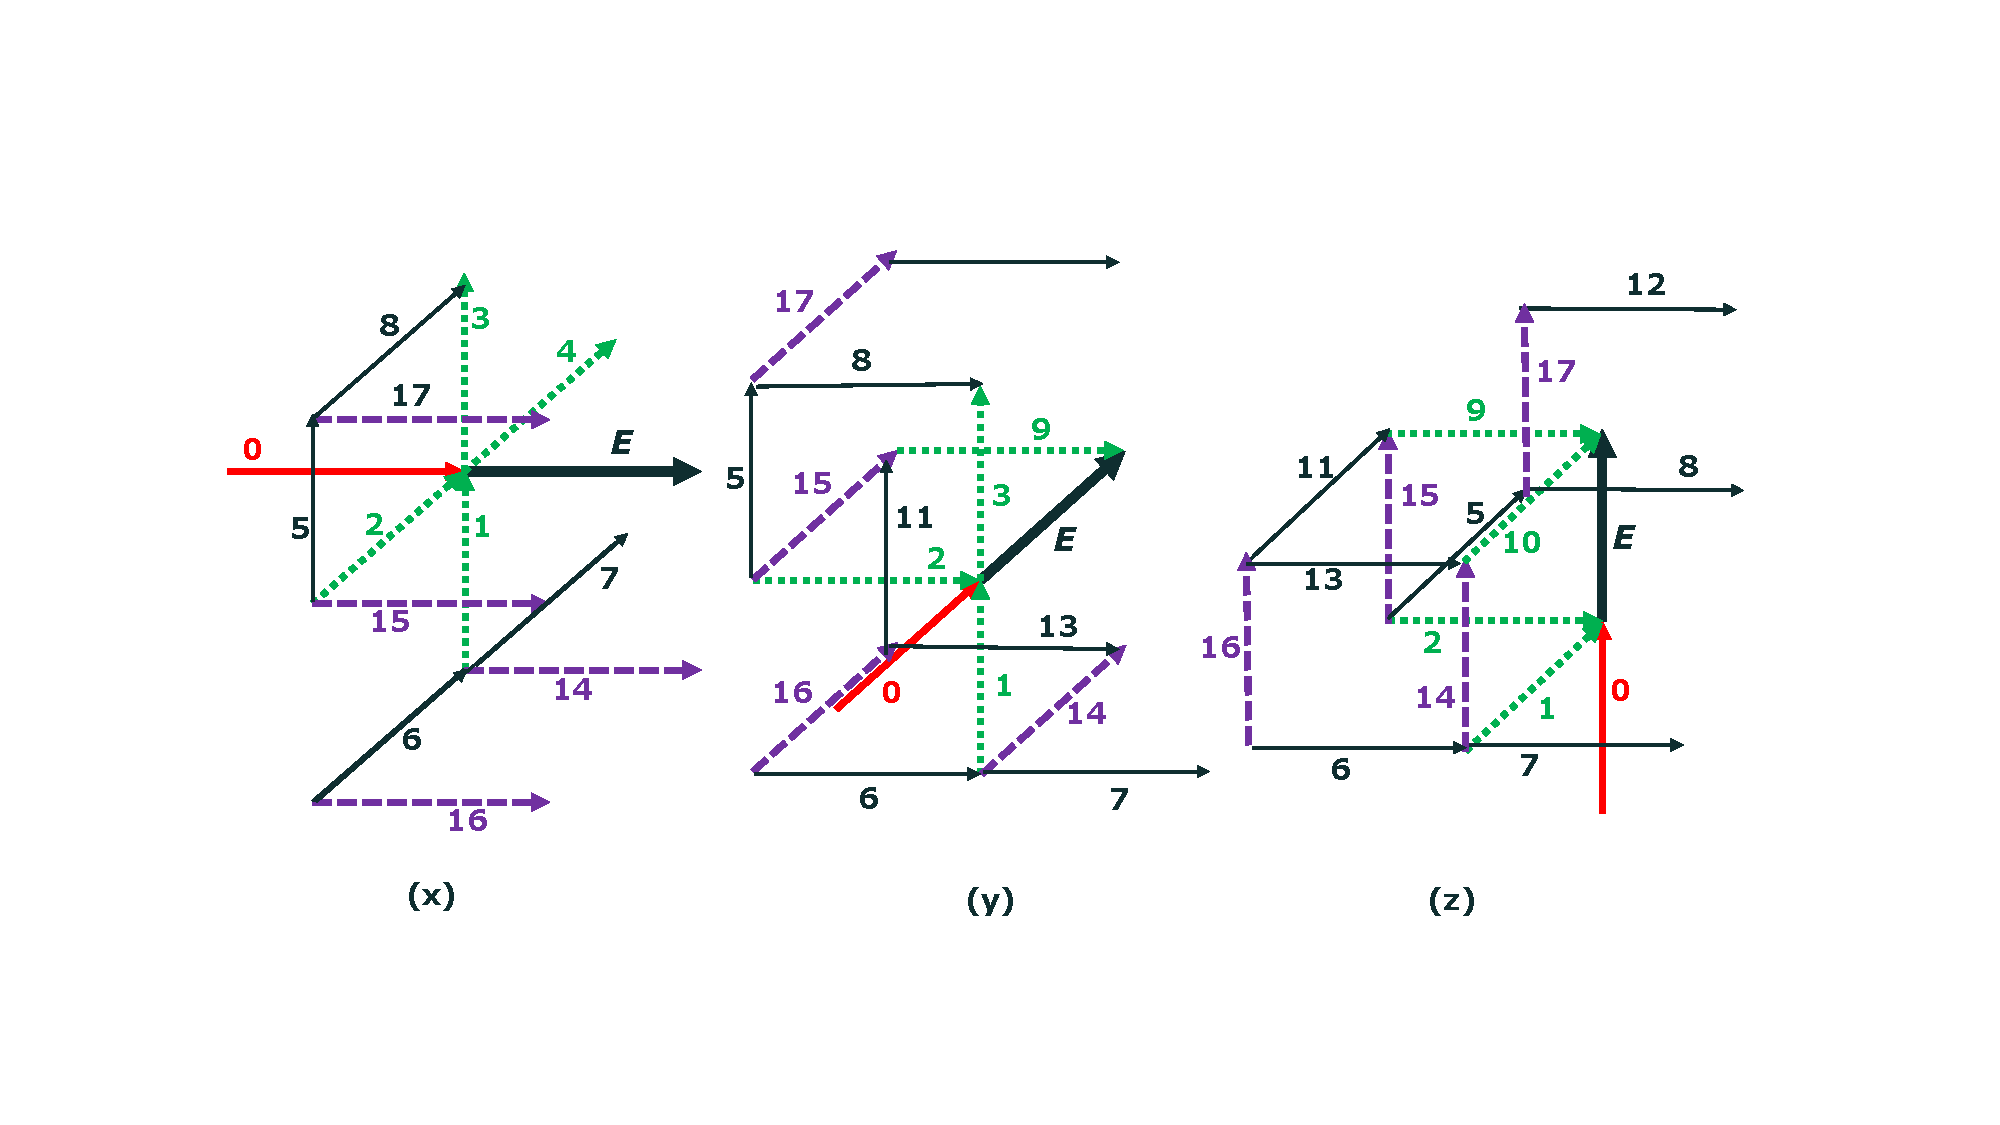
\includegraphics[scale=0.2]{image/18条边.pdf}
    }
    \hspace{0.1in}
    \subfloat[9条邻居边]{
        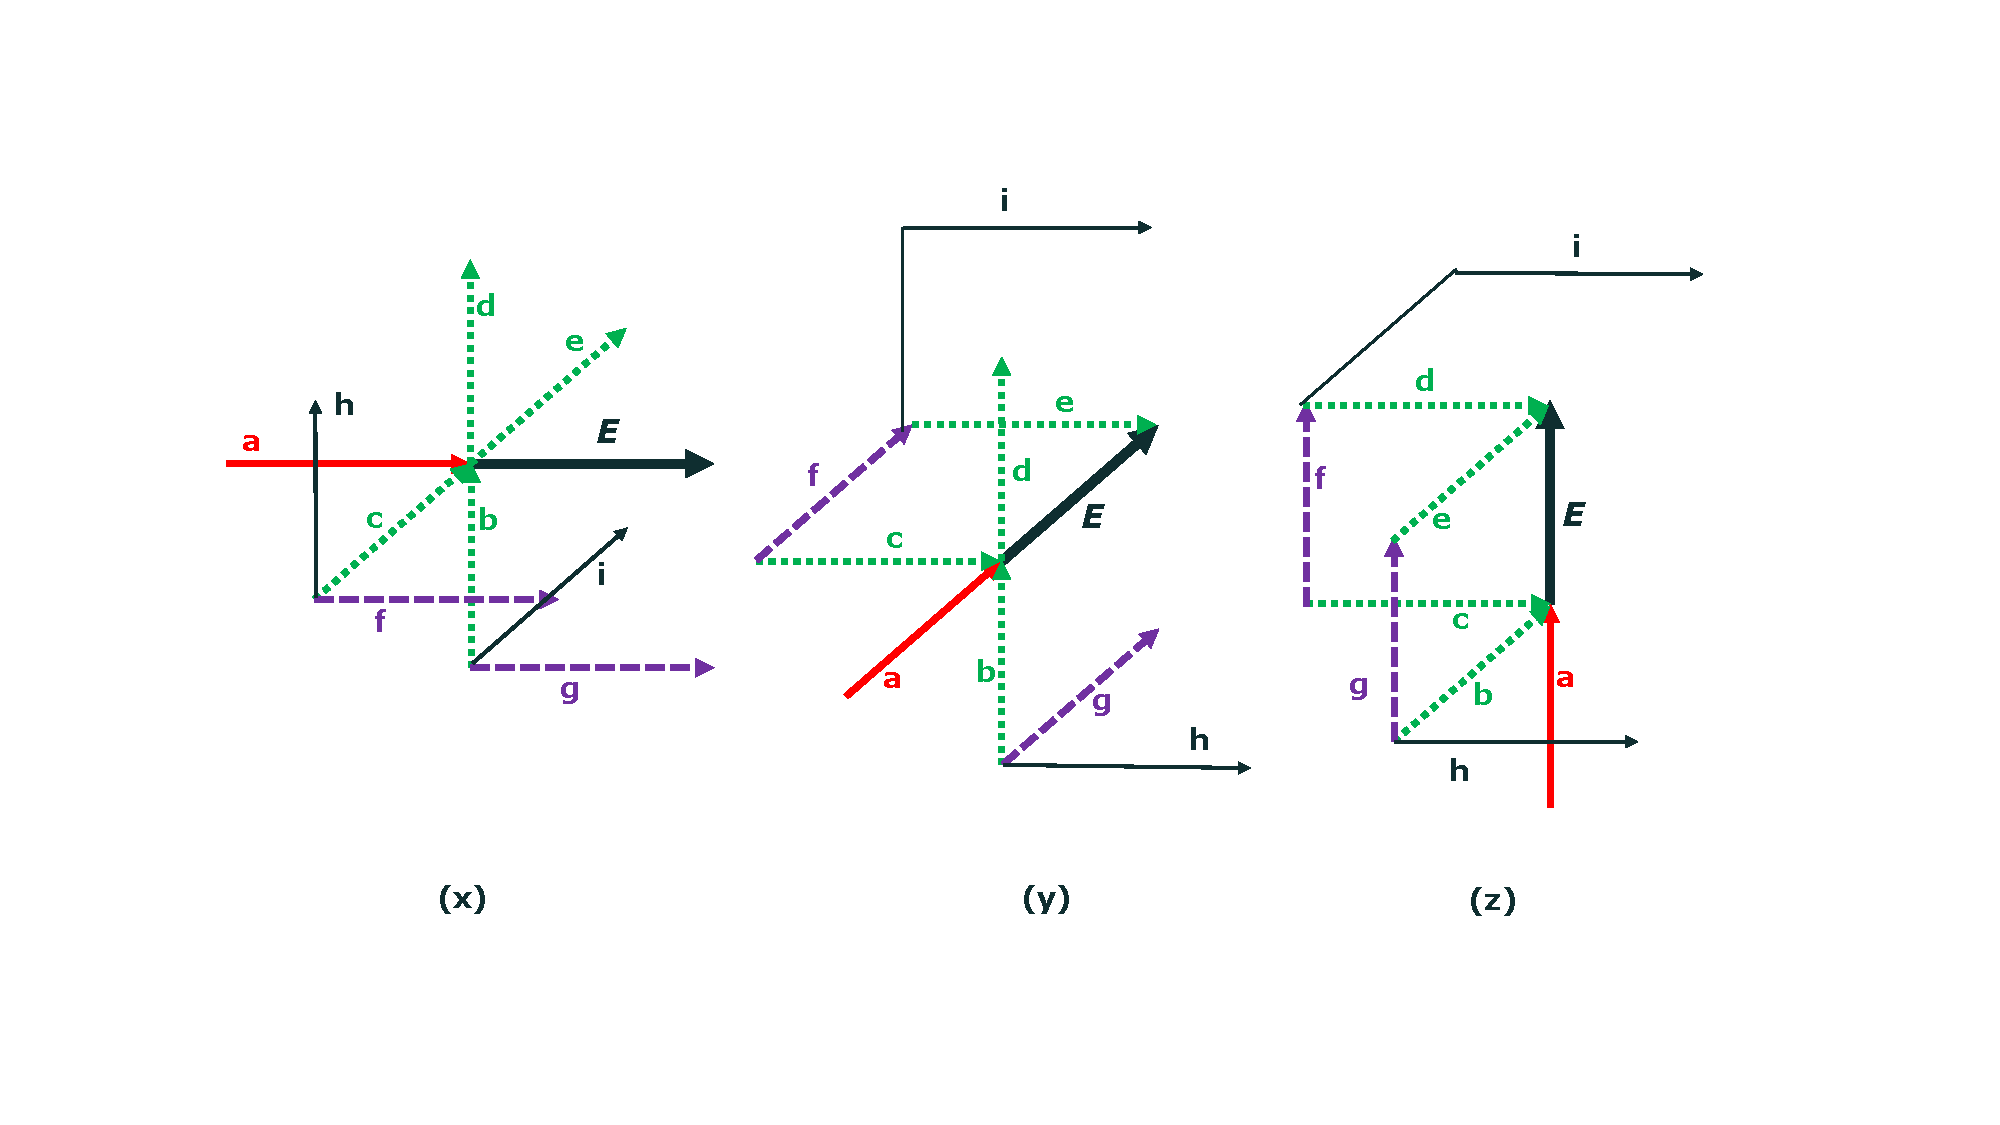
\includegraphics[scale=0.2]{image/9条边.pdf}
    }
    \caption{邻居边示意图}
    \label{fig:邻居边示意图}
\end{figure}
\\
\begin{figure}[htbp]
    %是可选项 h表示的是here在这里插入,t表示的是在页面的顶部插入
    \centering
    \subfloat[边的区间划分示意图]{
        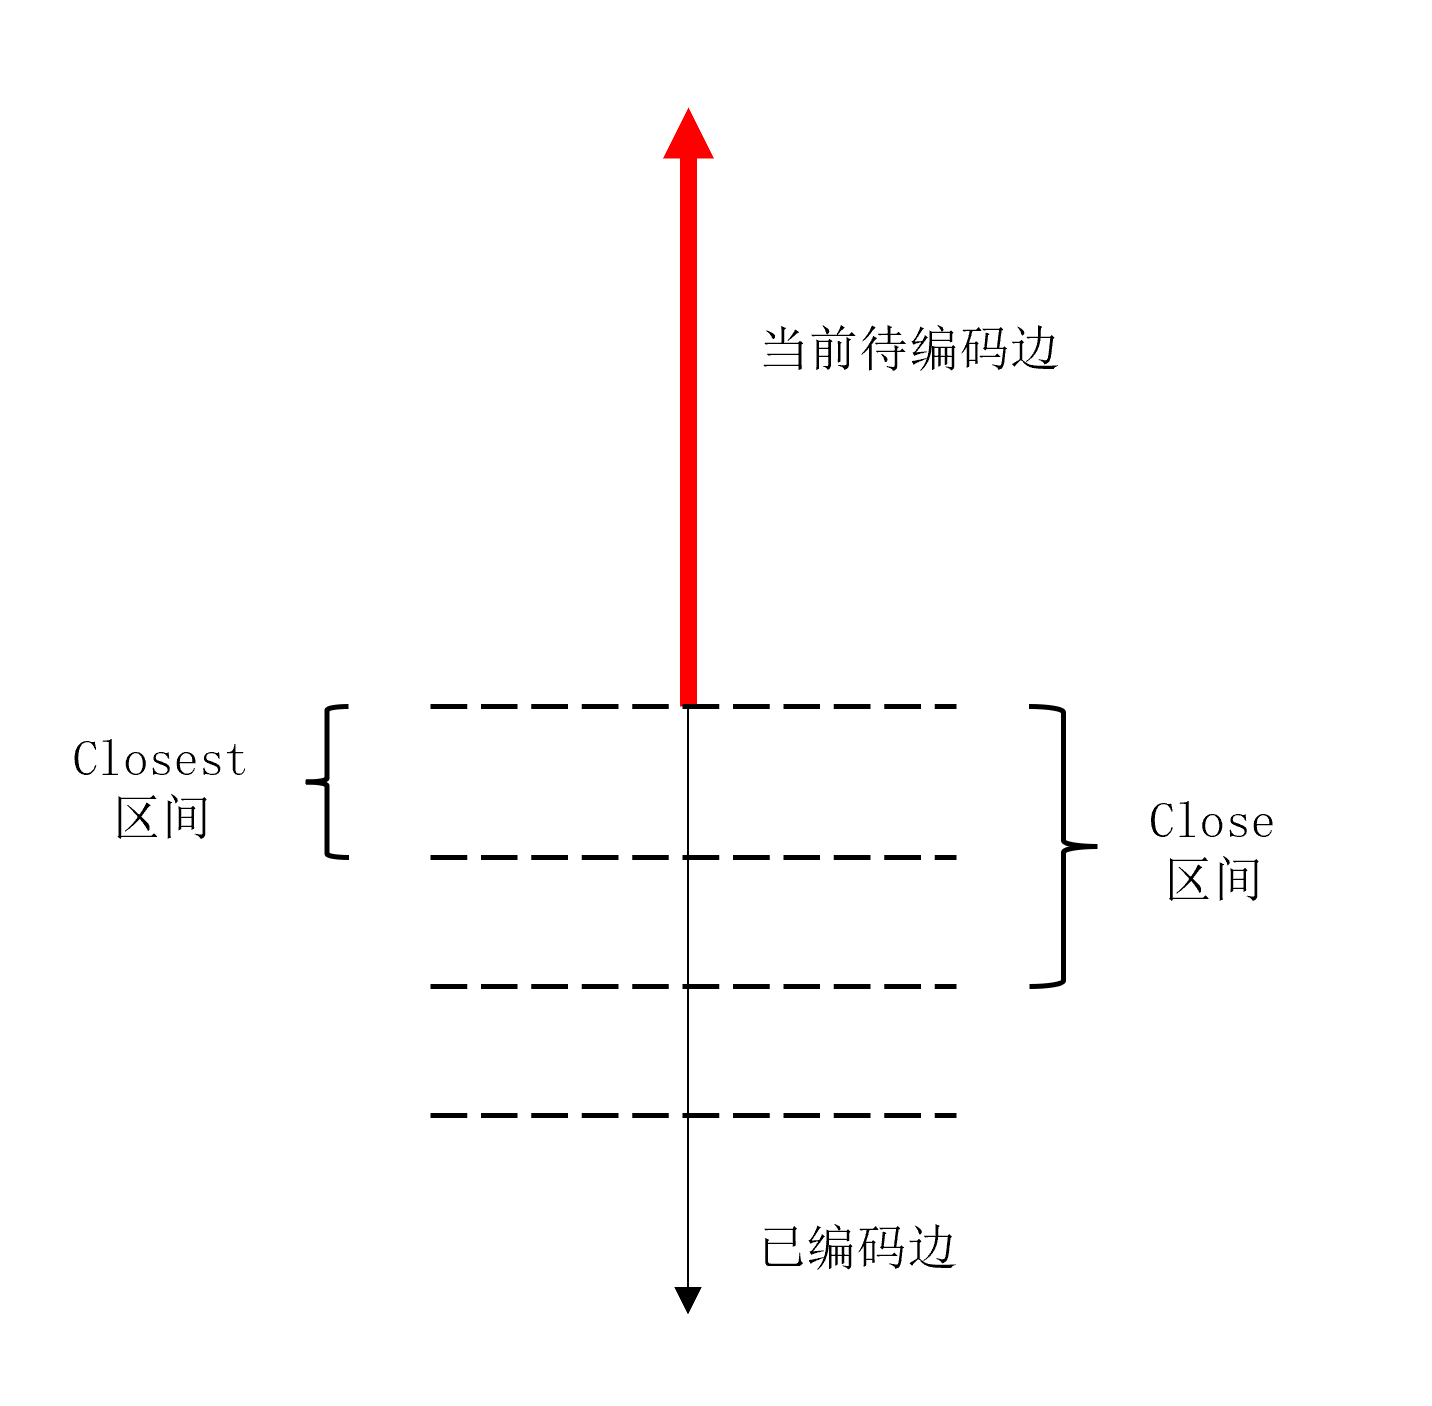
\includegraphics[scale=0.3]{image/区间划分示意图.png}
    }
    \hspace{0.2in}
    \subfloat[当前待编码边周围节点示意图]{
        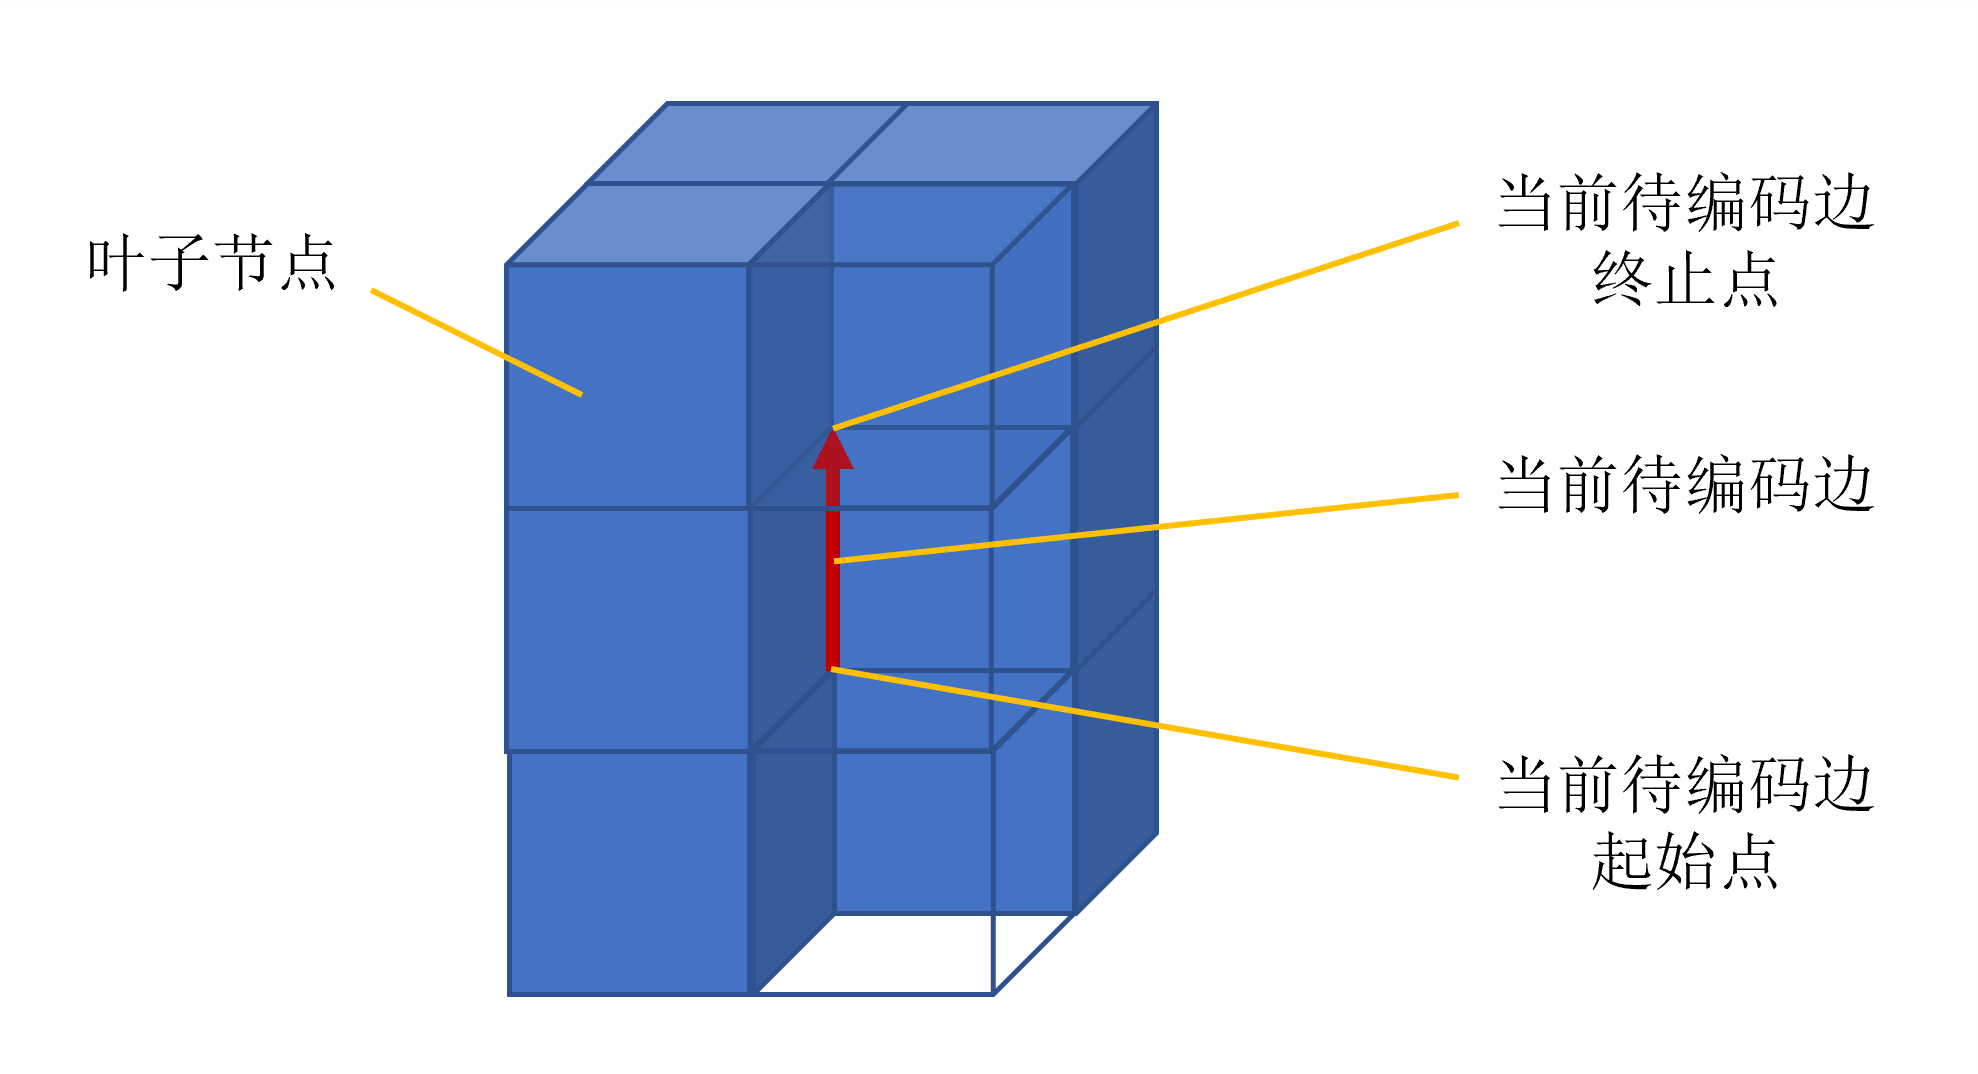
\includegraphics[scale=0.3]{image/当前待编码边周围节点.png}
    }
    \caption{上下文组成元素具体含义示意图}
    \label{fig:上下文组成元素的具体含义示意图}
\end{figure}

利用上述这些邻居边信息和邻居节点信息分别为编码顶点标识信息、顶点位置信息的高bit位以及顶点位置的低bit位构建了三套不同的上下文。其中强相关的信息作为上下文的主要信息,次相关的信息作为上下文的次要信息。
\begin{table}[h]
    \fontsize{10.5pt}{15pt}\selectfont
    \centering
    \caption{\label{tab1} 标识信息上下文编号}
    \begin{tabular}{cc}
        \toprule
        上下文名称                   & 编号 \\
        \midrule
        missedCloseStart             & ctx1 \\
        patternClosest  \& 1         & ctx2 \\
        direction                    & ctx3 \\
        patternClose \& (0b00011111) & ctx4 \\
        missedCloseStart             & ctx5 \\
        missedCloseStart             & ctx6 \\
        \bottomrule
    \end{tabular}
\end{table}

\subsection{顶点标识信息上下文}
顶点标识信息简而言之就是用1bit位来标识当前待编码边是否被占据,如果被占据则该bit置“1”,如果不被占据则该bit置“0”。其上下文结构如下:

1、主要信息组成
\begin{figure}[htbp]
    %是可选项 h表示的是here在这里插入,t表示的是在页面的顶部插入
    \centering
    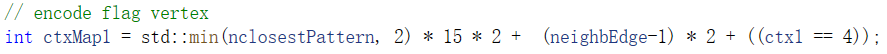
\includegraphics[scale=0.4]{image/flag主要信息组成.png}
    \caption{组成标识信息上下文的主要信息代码截图}
    \label{fig:flag主要信息组成}
\end{figure}

其中:

$nclosestPattern:$表示9条边中的前5条边在closest区间的数量。

$neighbEdge:$表示包含当前待编码边的 4 个节点的占据情况。

$ctx1:$表示包含当前待编码边起始点坐标的 4 个节点被占据的数量。
\\
\\
2、次要信息组成
\begin{figure}[htbp]
    %是可选项 h表示的是here在这里插入,t表示的是在页面的顶部插入
    \centering
    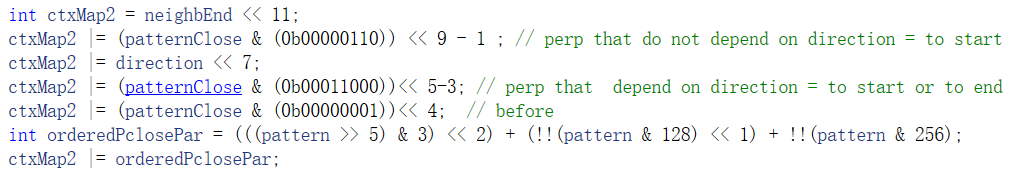
\includegraphics[scale=0.4]{image/flag次要信息组成.png}
    \caption{组成标识信息上下文的次要信息代码截图}
    \label{fig:flag次要信息组成}
\end{figure}

其中:

$neighbEnd$:表示包含当前待编码边终止点的 4 个节点的占据情况。

$patternClose$:9 条边在 close 区间被占据的情况。

$direction$:当前待编码边的朝向$(0=X,1=Y,2=Z)$。

$pattern$:9条边的被占据的情况。

另外,如表\ref{tab1}所示,本文按照次要信息的现有上下文顺序对其进行编号。

\subsection{顶点位置信息上下文}
在编码叶子节点中某一条被占据边上的顶点坐标时,首先需要对顶点坐标进行量化操作,现有的量化操作是将顶点坐标量化为0,1,2,3四个坐标值,因此需要用2bit来表示量化后的顶点位置信息。由于两个bit位所承载的位置信息在物理含义上不一致,对于高bit位,它将量化后的顶点坐标可选范围缩减一半,顶点坐标取值要么为0,1要么为2,3;低bit位则是在高bit位基础上,完全确定顶点坐标位置。因此分别为其构建不同的上下文模型。

对于高bit位:

1、主要信息组成

\begin{figure}[htbp]
    %是可选项 h表示的是here在这里插入,t表示的是在页面的顶部插入
    \centering
    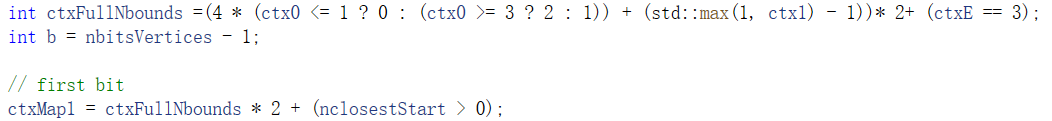
\includegraphics[scale=0.4]{image/position1主要信息组成.png}
    \caption{组成位置信息上下文高bit的主要信息代码截图}
    \label{fig:position1主要信息组成}
\end{figure}

其中:

$ctx0$:表示包含当前待编码边终止点坐标的 4 个节点被占据的数量。

$ctxE$:表示当前待编码边周围4各个节点被占据数量

$nclosestStart$:表示9条边中的前5条边在closest区间被占据的数量


2、次要信息组成

\begin{figure}[htbp]
    %是可选项 h表示的是here在这里插入,t表示的是在页面的顶部插入
    \centering
    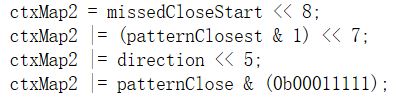
\includegraphics[scale=0.4]{image/position1次要信息组成.png}
    \caption{组成位置信息上下文高bit的次要信息代码截图}
    \label{fig:positon1次要信息组成}
\end{figure}

其中:

missedCloseStart:表示4条相邻垂直边不被占据的数量

patternClosest:表示9条边在closest区间被占据的情况

对于低bit位,其上下文模型的主要信息部分与高bit位一致,主要差别体现在次要信息更加丰富。下面给出该bit位上下文模型的次要信息组成:

\begin{figure}[htbp]
    %是可选项 h表示的是here在这里插入,t表示的是在页面的顶部插入
    \centering
    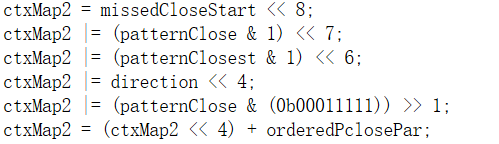
\includegraphics[scale=0.4]{image/position2次要信息组成.png}
    \caption{组成位置信息上下文低bit的次要信息代码截图}
    \label{fig:position2次要信息组成}
\end{figure}

其中:

orderedPclosePar:表示不相邻的垂直边与平行边的占据情况

同样的对次要信息上下文按照其现有使用顺序进行编号,如表\ref{tab2}所示。
\begin{table}[h]
    \fontsize{10.5pt}{15pt}\selectfont
    \centering
    \caption{\label{tab2} 位置信息上下文编号}
    \begin{tabular}{ccc}
        \toprule
        位置信息             & 上下文名称                      & 编号 \\
        \midrule
        \multirow{4}*{高bit} & missedCloseStart                & ctx1 \\
                             & patternClosest  \& 1            & ctx2 \\
                             & direction                       & ctx3 \\
                             & patternClose \& (0b00011111)    & ctx4 \\
        \midrule
        \multirow{6}*{低bit}
                             & missedCloseStart                & ctx1 \\
                             & patternClose    \& 1            & ctx2 \\
                             & patternClosest  \& 1            & ctx3 \\
                             & direction                       & ctx4 \\
                             & patternClose    \& (0b00011111) & ctx5 \\
                             & orderedPclosePar                & ctx6 \\
        \bottomrule
    \end{tabular}
\end{table}

对于要编码的顶点标识信息与位置信息,有了这一系列的上下文模型后,采用动态OBUF技术进行熵编码操作,就可以达到去除点云空间坐标之间冗余信息的目的,从而有效降低了的码流大小,提高了编码效率。
\section{上下文信息熵测量}
\label{上下文信息熵测量}
虽然利用基于动态OBUf的熵编码技术能够有效的降低码流,但是其是否动态更新次要信息是通过判断当前已使用的上下文模型被选中的次数是否大于一定阈值来控制的,因此本文希望通过计算各个上下文的信息熵大小,来决定整套上下文模型的第一个上下文。其中依据的原理是,若某一上下文熵值越小,则说明它与当前待编码边的相关性越强,因此如果将其放在越高bit位使用,随着熵编码过程的进行,所选择的熵编码器概率模型会越来越符合当前待编码值的实际概率分布,整个熵编码过程更加高效。基于这一理论,本节尝试对三组次要信息所有用到的所有上下文进行信息熵的测量与对比,从而选出最佳的第一上下文。

本文探究如何生成求解信息熵的可执行文件是在$basketball\_player\_vox11\_00000200$序列的$r01$码率点上进行的,首先在TMC13v20的参考代码中加入如图\ref{fig:键值对}所示的键值对,用于存储各上下文信息不同值与当前待编码bit不同值之间的匹配数量。
\begin{figure}[htbp]
    %是可选项 h表示的是here在这里插入,t表示的是在页面的顶部插入
    \centering
    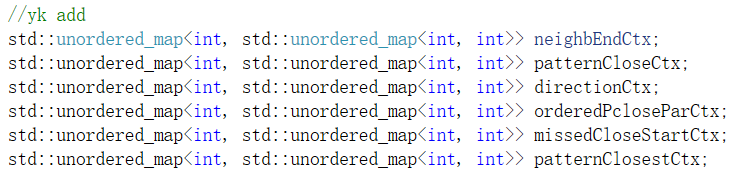
\includegraphics[scale=0.4]{image/键值对.png}
    \caption{键值对代码截图}
    \label{fig:键值对}
\end{figure}

例如计算标识信息时用到的键值对:$std::unordered_map<int, std::unordered_map<int, int>> directionCtx$存储了$direction$的3个不同取值0,1,2与当前待编码边是否被占据的0,1信息匹配的所有情况各自的次数,利用该键值对存储的数据,可以得到$direction=0$时,当前待编码边占据时的占比$rate1$与不占据时的占比$rate0$,同时也可以得到$direction=0$在该类上下文中的占比$countRate$。基于这些数据,利用如下信息熵求解公式\ref{fig:信息熵求解}:
\begin{equation}
    entropy = rate0*\log \frac{1}{{rate0}} + rate1*\log \frac{1}{{rate1}}
    \label{fig:信息熵求解}
\end{equation}
可以得出该类上下文在direction=0时,它的信息熵如公式\ref{fig:信息熵2}所示。
\begin{equation}
    entropy0 = entropy*countRate
    \label{fig:信息熵2}
\end{equation}

同理,$direction=1$和$direction=2$时,可以求出其对应的信息熵$entropy1$,$entropy2$.由此便得到了direction这类上下文的信息熵$entropy=entropy0+entropy1+entropy2$。重复这一计算过程,可以求得编码顶点标识信息
时用到的各类上下文的信息熵。对于其他序列其他码率点的测试,本文采取的方法是:

1、将上述计算方法写入TMC13v20的参考代码,并且在参考代码中加入打印每个slice求得的信息熵的代码后生成可执行文件。

2、撰写python脚本文件将可执行文件用于通测最终测试性能所需的所有点云序列的所有码率点,并将得到的数据结构用txt文本输出。

3、撰写python脚本对所有生成的txt文本进行遍历,获取其中的信息熵并按不同序列的不同码率点输出到excel表格中。其中对于同一码率点的不同slice,将不同slice得到的信息熵进行简单平均作为该码率点的信息熵。

4、重复上述步骤,得到所有测试点云序列的全部码率点下的各类上下文信息熵。

5、最后进行折线图绘制,并分析结果。

以标识信息为例,从四类测试点云序列(solid,dense,sparse,scant)中各取一个测试序列作图,得到其次要信息所用到的上下文的信息熵对比图如\ref{fig:信息熵对比图}所示。

\begin{figure}[h]
    %是可选项 h表示的是here在这里插入,t表示的是在页面的顶部插入
    \centering
    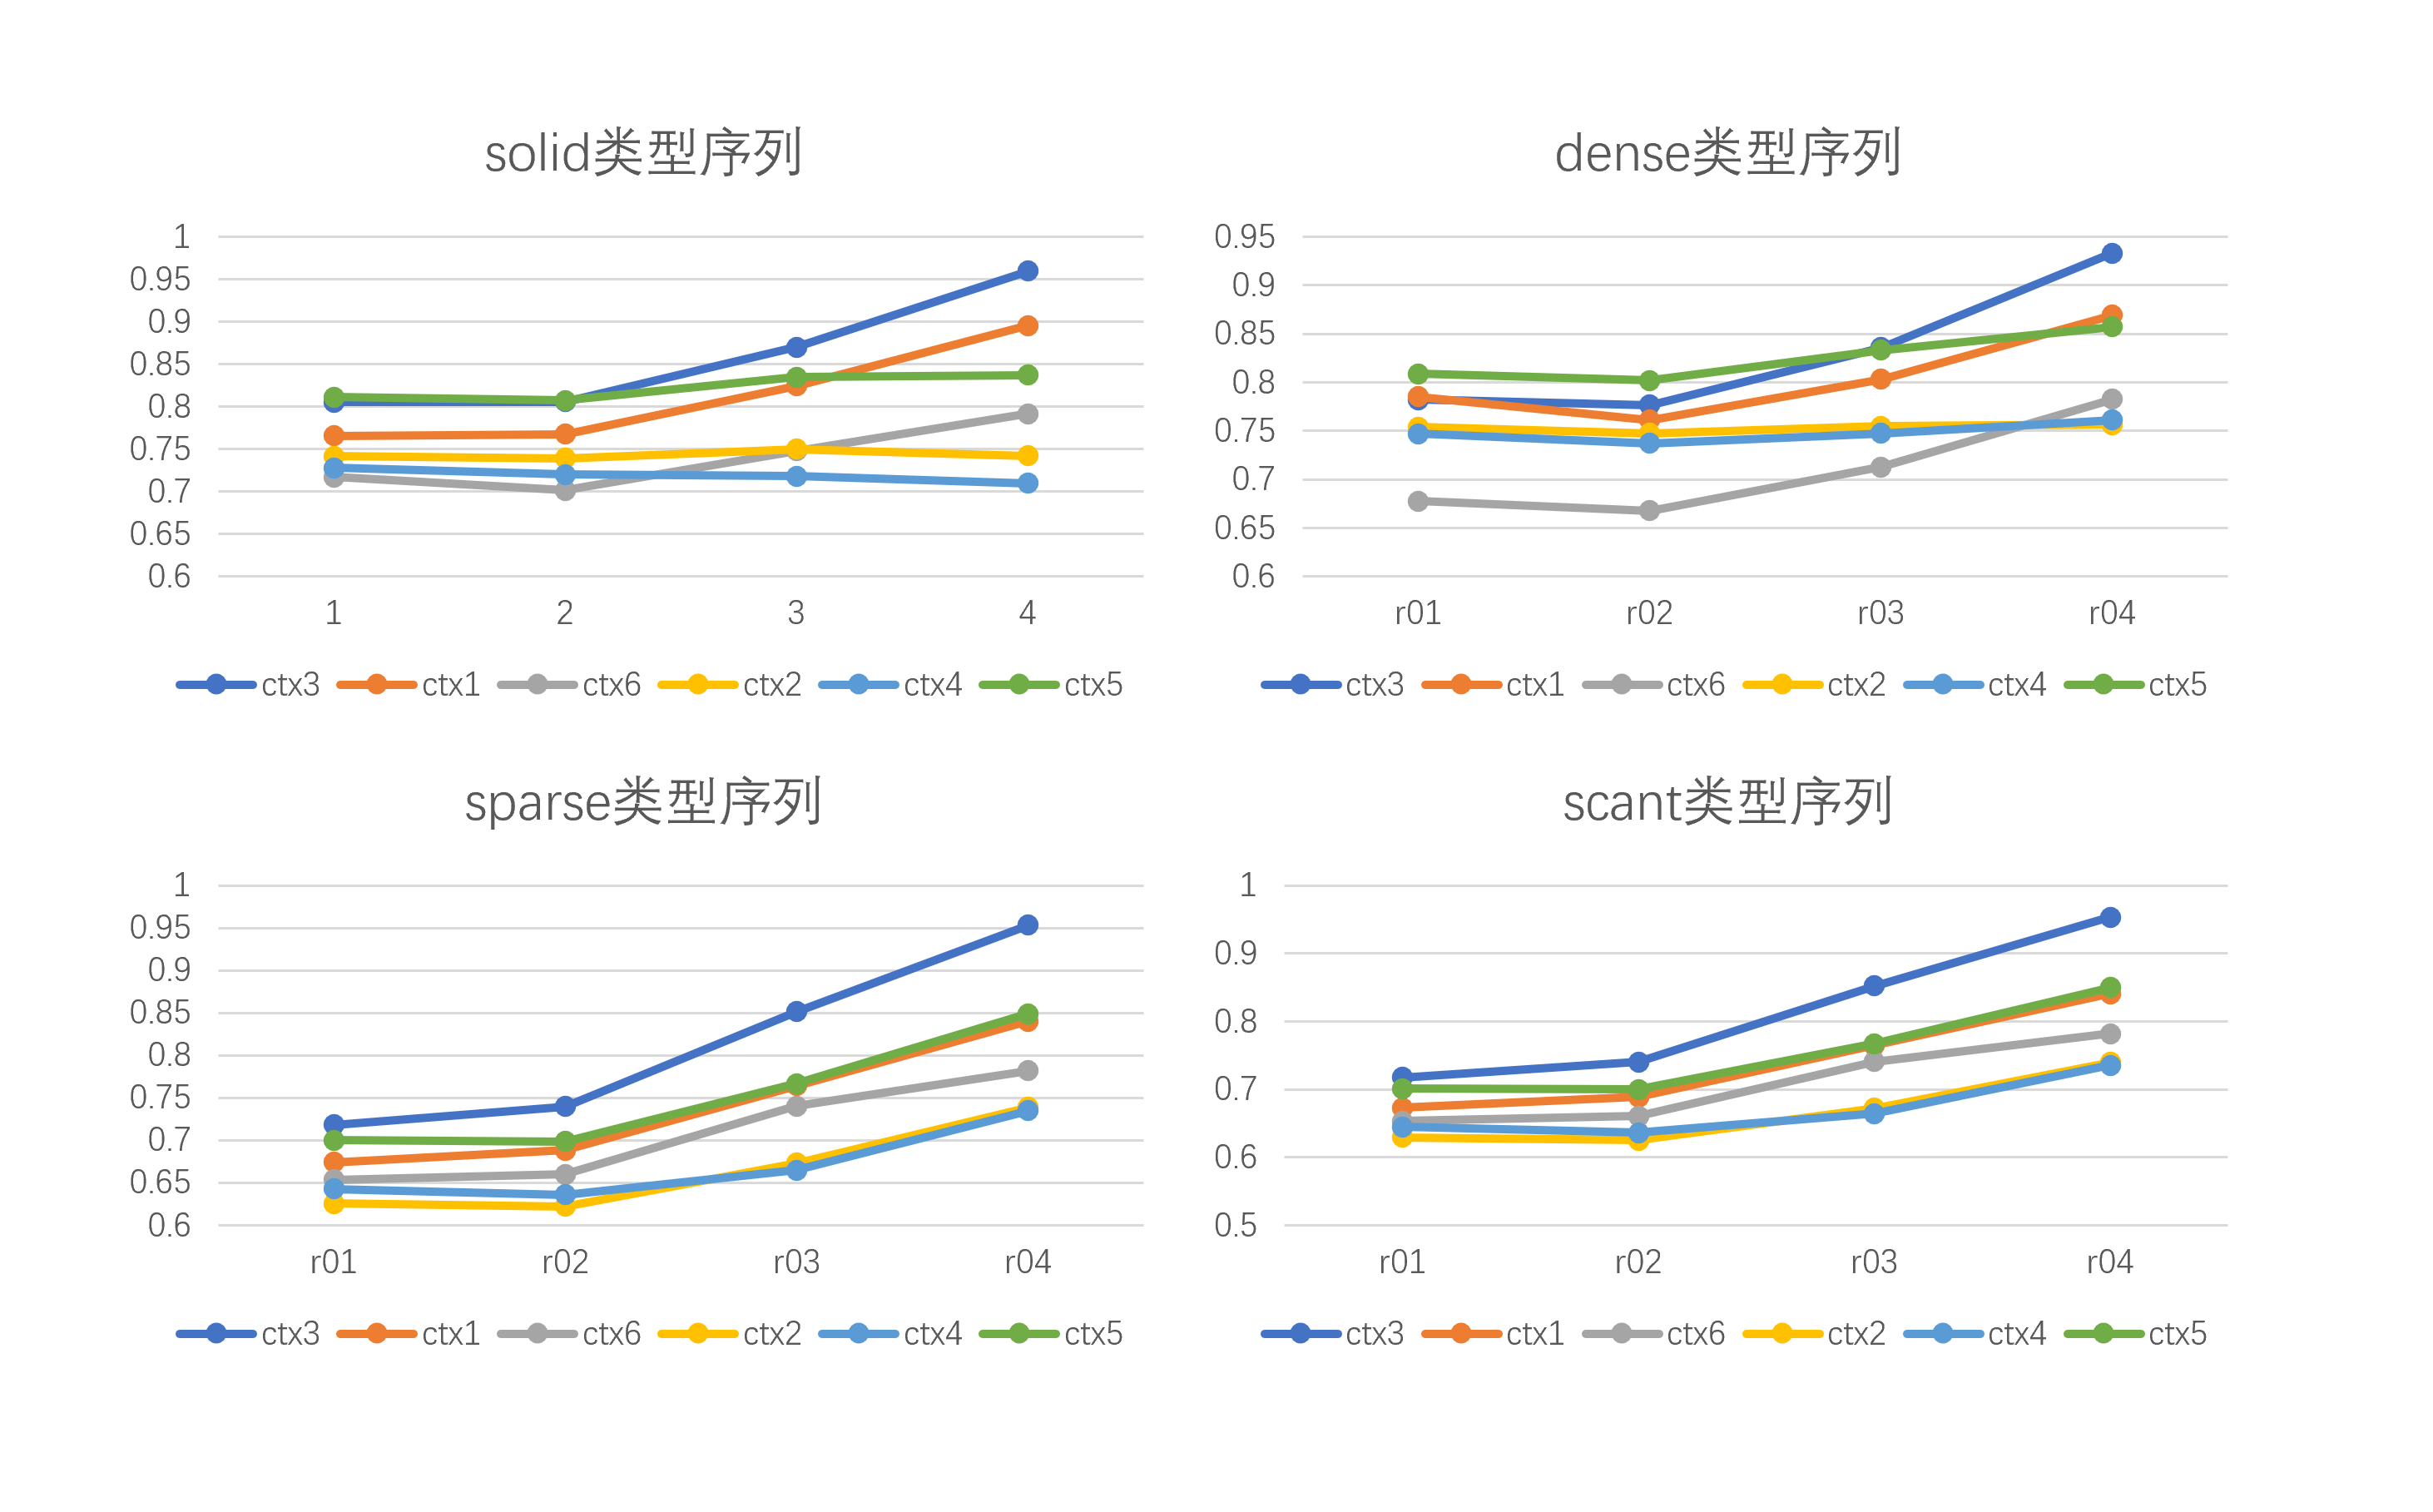
\includegraphics[scale=0.4]{image/flag信息熵对比图.png}
    \caption{标识信息的信息熵对比图}
    \label{fig:信息熵对比图}
\end{figure}

图中我们可以看出在各类点云序列下,ctx4这一上下文基本处于最低熵值的位置,故选取ctx4,即patternClose\&(0b00011000)作为编码顶点标识信息所用到的次要信息的第一个上下文。

同理,对编码顶点位置信息用到的次要信息所包含的上下文信息熵进行测试,可得到如图\ref{fig:位置信息上下文的信息对比图}所示结果。据此得出高bit位应选取ctx4,即patternClose\&(0b00011111)作为其第一类上下文;低bit位应选取ctx5,即patternClose\& (0b00011111)作为其第一类上下文。
\begin{figure}[h]
    %是可选项 h表示的是here在这里插入,t表示的是在页面的顶部插入
    \centering
    \subfloat[高bit位]{
        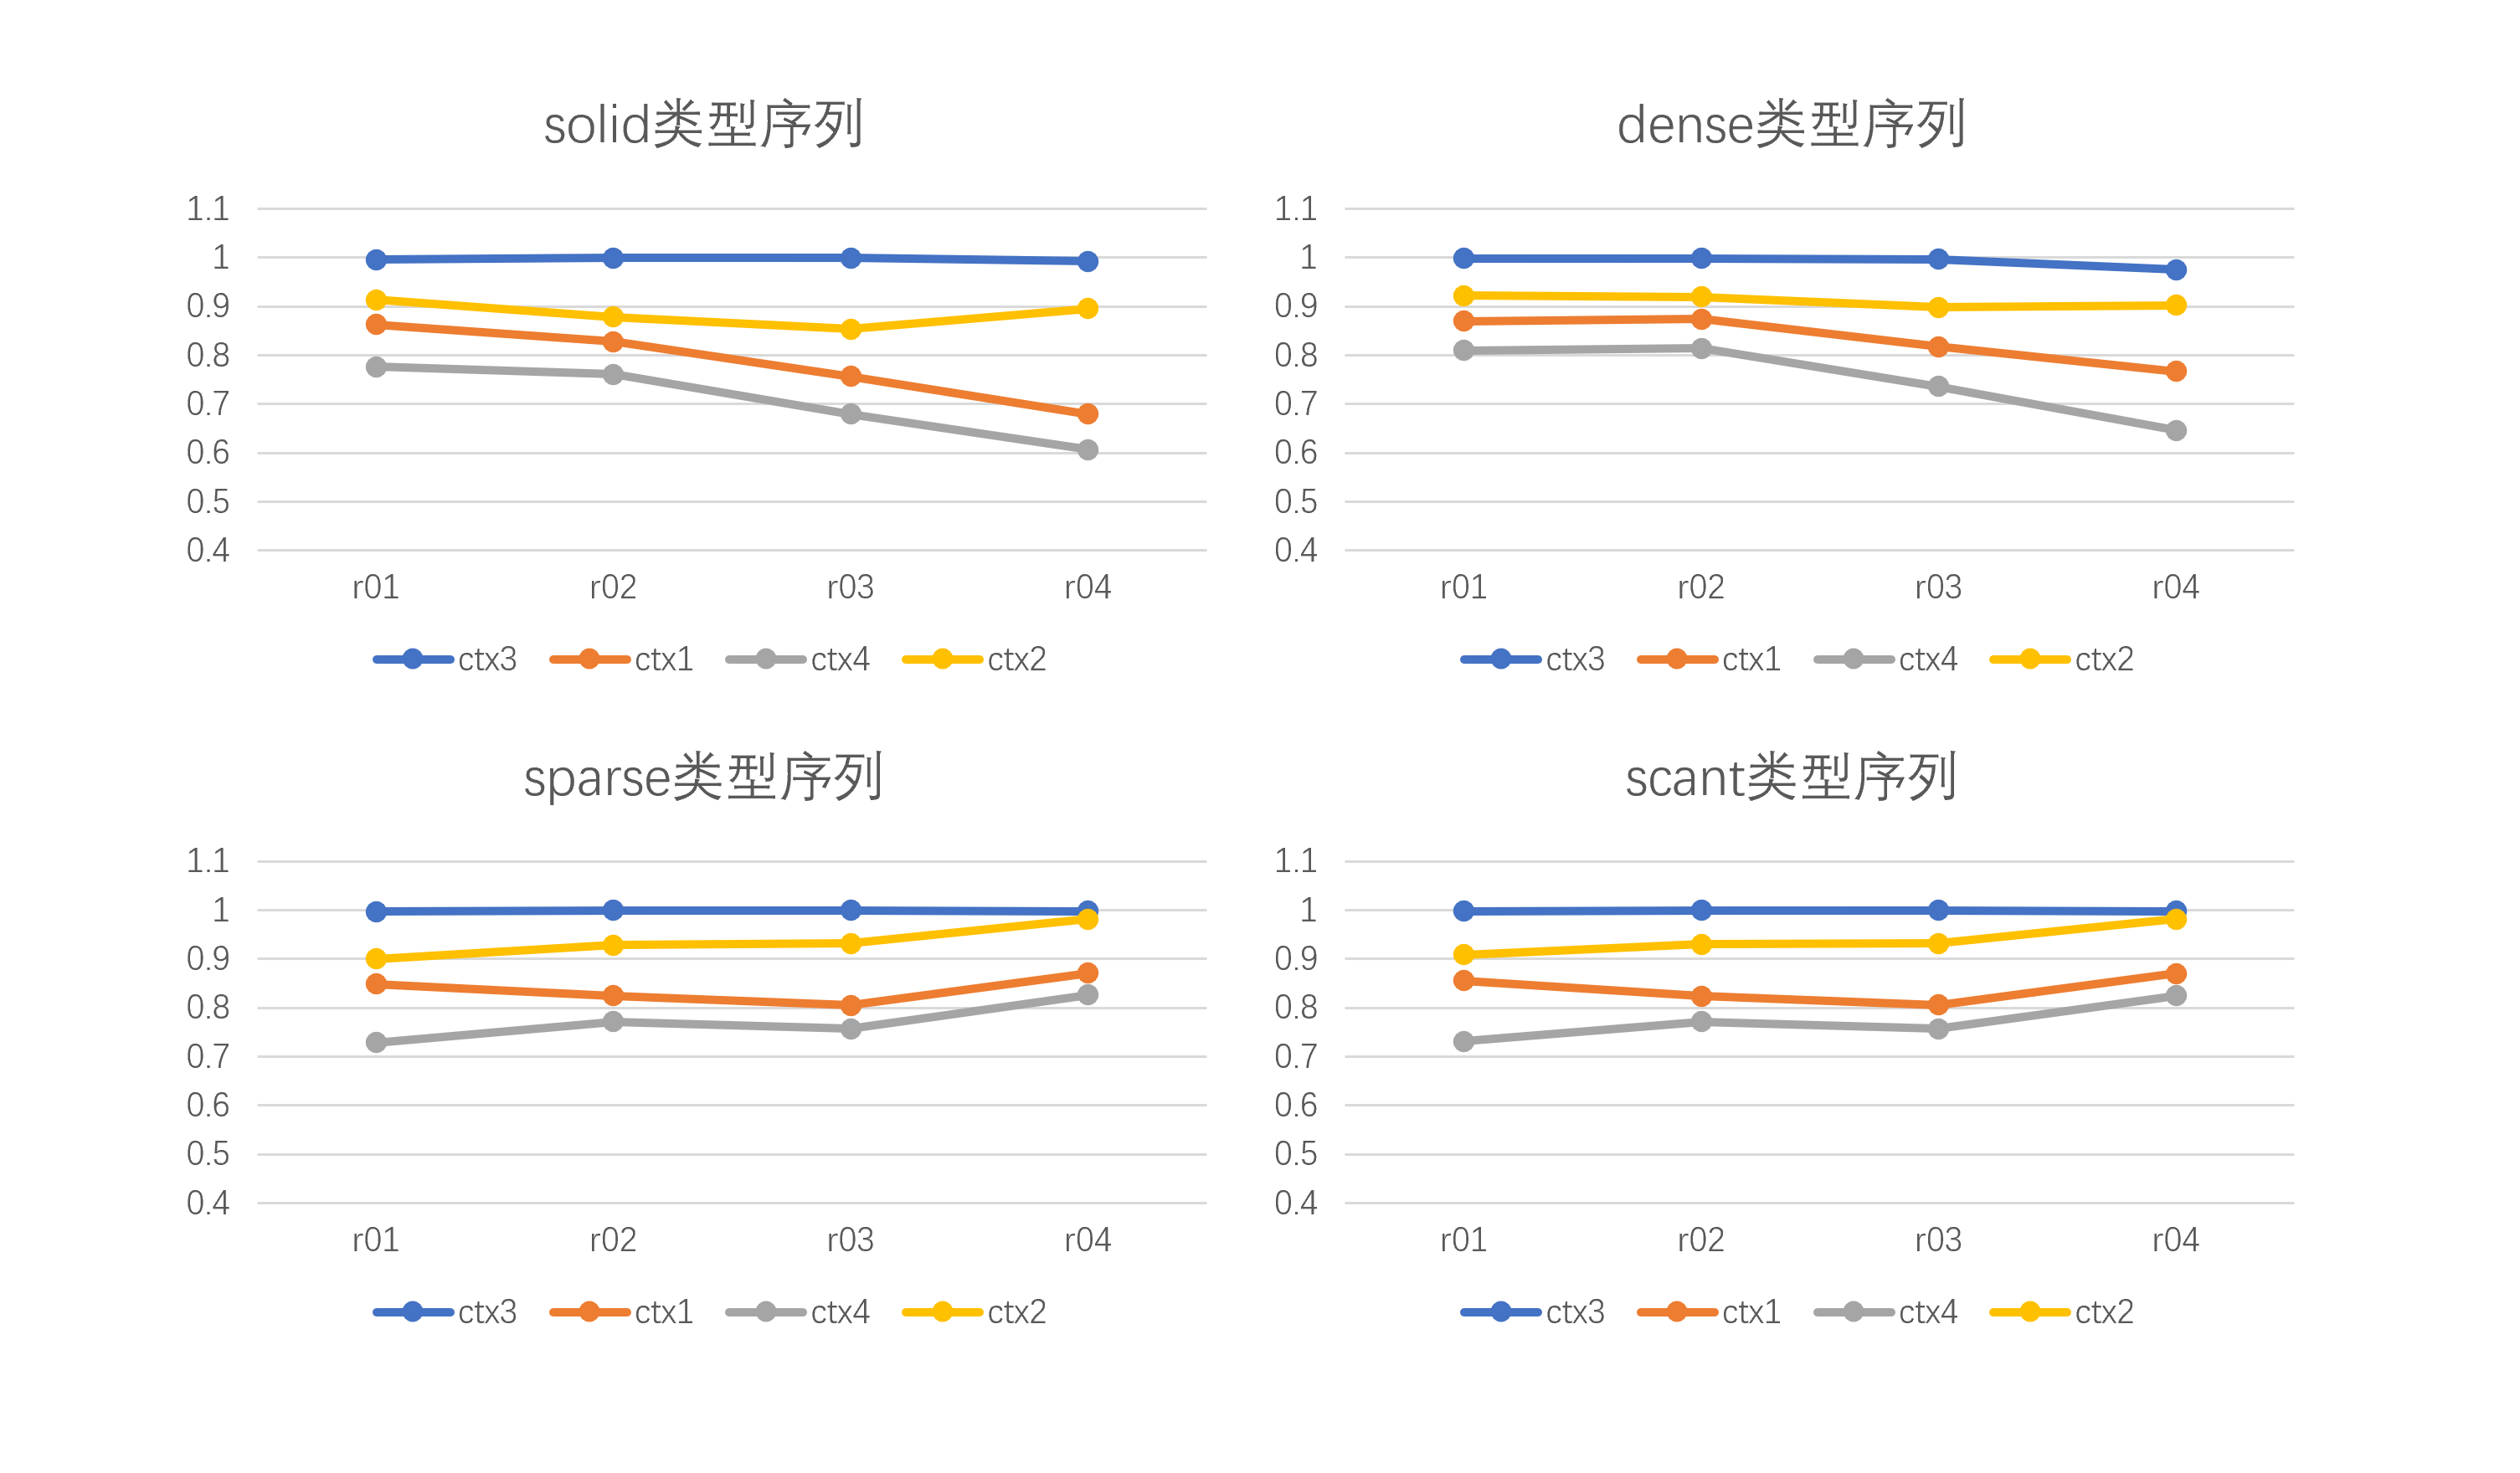
\includegraphics[scale=0.4]{image/高bit位置信息的信息熵.png}
    }
    \hspace{0.1in}
    \subfloat[低bit位]{
        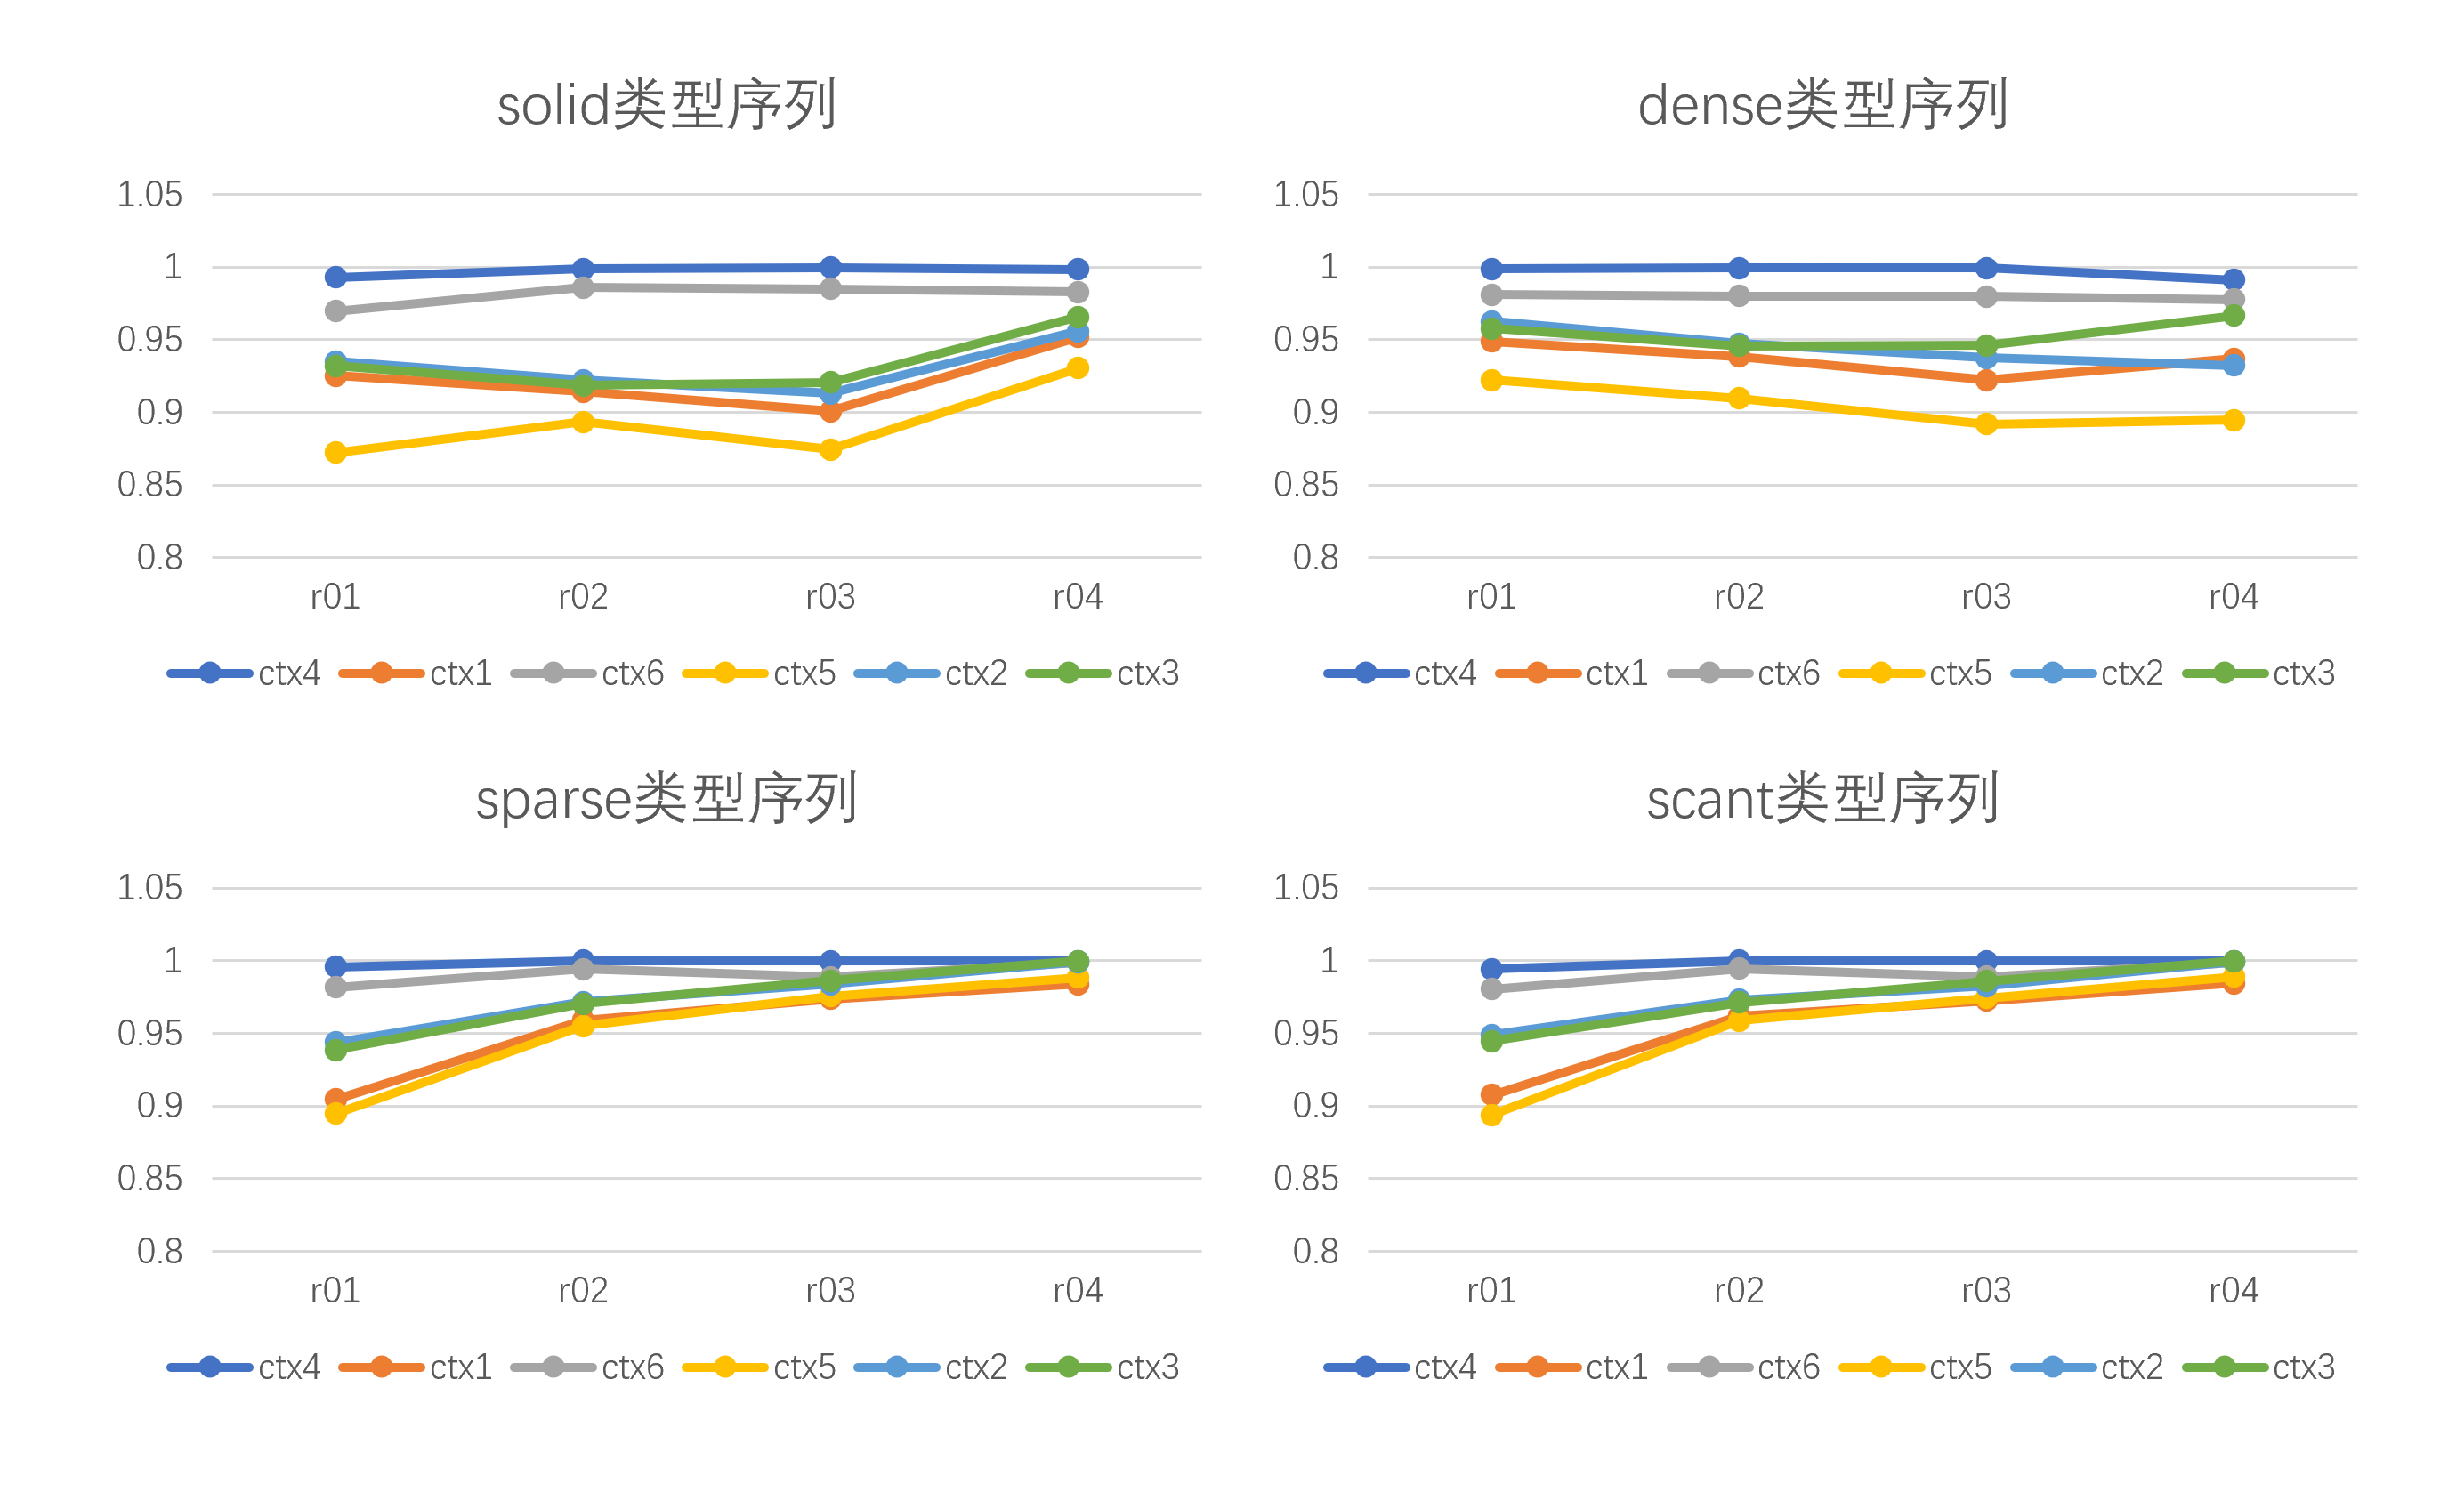
\includegraphics[scale=0.4]{image/低bit位置信息的信息熵.png}
    }
    \caption{位置信息的信息熵对比图}
    \label{fig:位置信息上下文的信息对比图}
\end{figure}
\section{上下文条件熵测量}
基于熵越小,上下文与当前待编码边相关性越强的理论基础,本文在三套上下文的第一类上下文已经确定的基础上对剩余上下文的条件熵进行测试,进而得到三套上下文模型的局部最优顺序。本文条件熵的测试将在$basketball\_player\_vox11\_00000200$序列的$r01$码率点下进行。

以标识信息的上下文条件熵测量为例。依据信息熵的测量结果将$ctx4$作为首要条件,在此条件下对剩余上下文进行条件熵的测试。实际操作过程中,先将$ctx4$分别与剩余五类上下文进行组合构成五类新的上下文,如图\ref{上下文新组合}所示。

\begin{figure}[h]
    %是可选项 h表示的是here在这里插入,t表示的是在页面的顶部插入
    \centering
    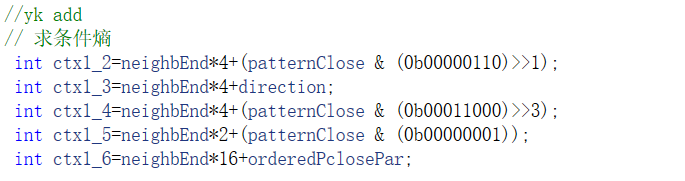
\includegraphics[scale=0.4]{image/上下文新组合.png}
    \caption{组合测试所需上下文部分代码截图}
    \label{上下文新组合}
\end{figure}

从而将对条件熵的测量转换为了对这新的五类熵下文进行信息熵的测量,目的是可以继续使用\ref{上下文信息熵测量}节所介绍的方法。如图\ref{标识信息条件熵}所示,具体实验过程如下:
\begin{figure}[h]
    %是可选项 h表示的是here在这里插入,t表示的是在页面的顶部插入
    \centering
    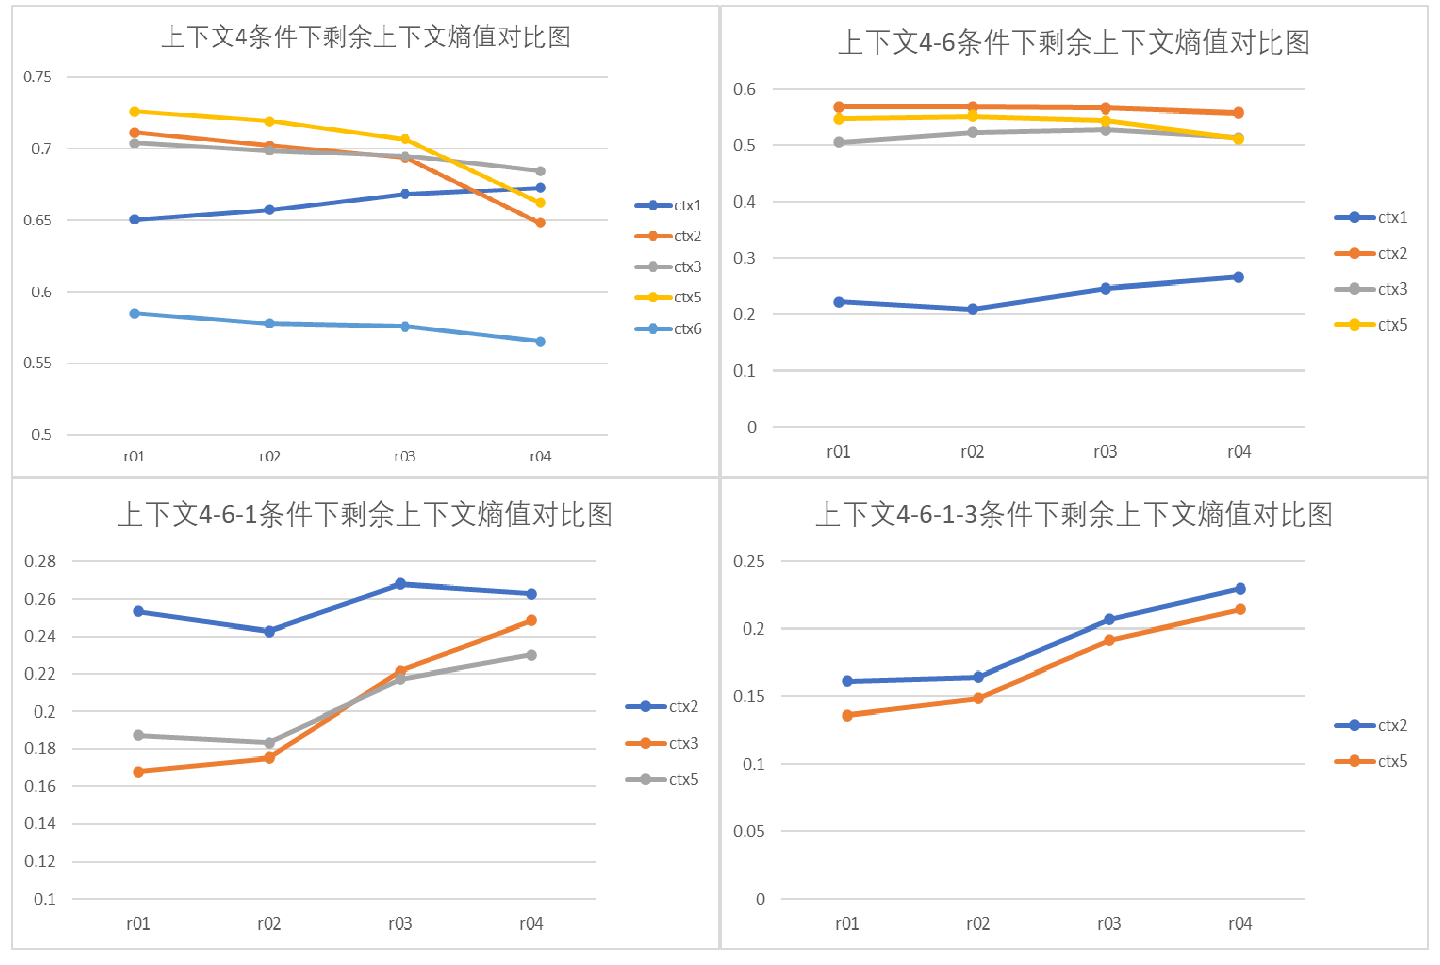
\includegraphics[scale=0.5]{image/标识信息条件熵.pdf}
    \caption{标识信息条件熵对比图}
    \label{标识信息条件熵}
\end{figure}

1、以ctx4作为条件时,测试得到剩余五类上下文的条件熵,得到ctx6条件熵在四个码率点下均明显小于其他四类上下文条件熵,因此选择ctx6作为第二个条件。

2、以ctx4、ctx6作为条件时,测试得到剩余四类上下文的条件熵,得到ctx1条件熵在四个码率点下明显小于其他三类上下文条件熵,因此选择ctx1作为第三个条件。

3、以ctx4、ctx6、ctx1作为条件时,测试得到剩余三类上下文的条件熵。此时得到ctx3在r01与r02码率点下条件熵低于ctx5,但是在r03与r04码率点下,ctx3的条件熵比ctx5的条件熵高。对于这种情况,将四个码率点的条件熵取平均,然后比较其大小。最终得出ctx3在此条件下四个码率点的平均条件熵要小于ctx5,因此选择cxt3作为第四个条件。

4、至此,仅剩下ctx2与ctx5未进行测试,在先前四类上下文的条件下,测量其条件熵,得到ctx5条件在四个码率点小均明显小于ctx2条件熵,因此ctx5将在ctx2前作为上下文被使用。

最终得到编码顶点标识信息时,其次要信息所包含的上下文的顺序应为ctx4-ctx6-ctx1-ctx3-ctx5-ctx2。

对于2bit位置信息,它们条件熵的具体测试过程与标识信息一致,在此不再赘述,给出其测试过程的条件熵对比图如\ref{位置信息条件熵对比图}所示。

\begin{figure}[h]
    %是可选项 h表示的是here在这里插入,t表示的是在页面的顶部插入
    \centering
    \subfloat[高bit位置信息条件熵对比图]{
        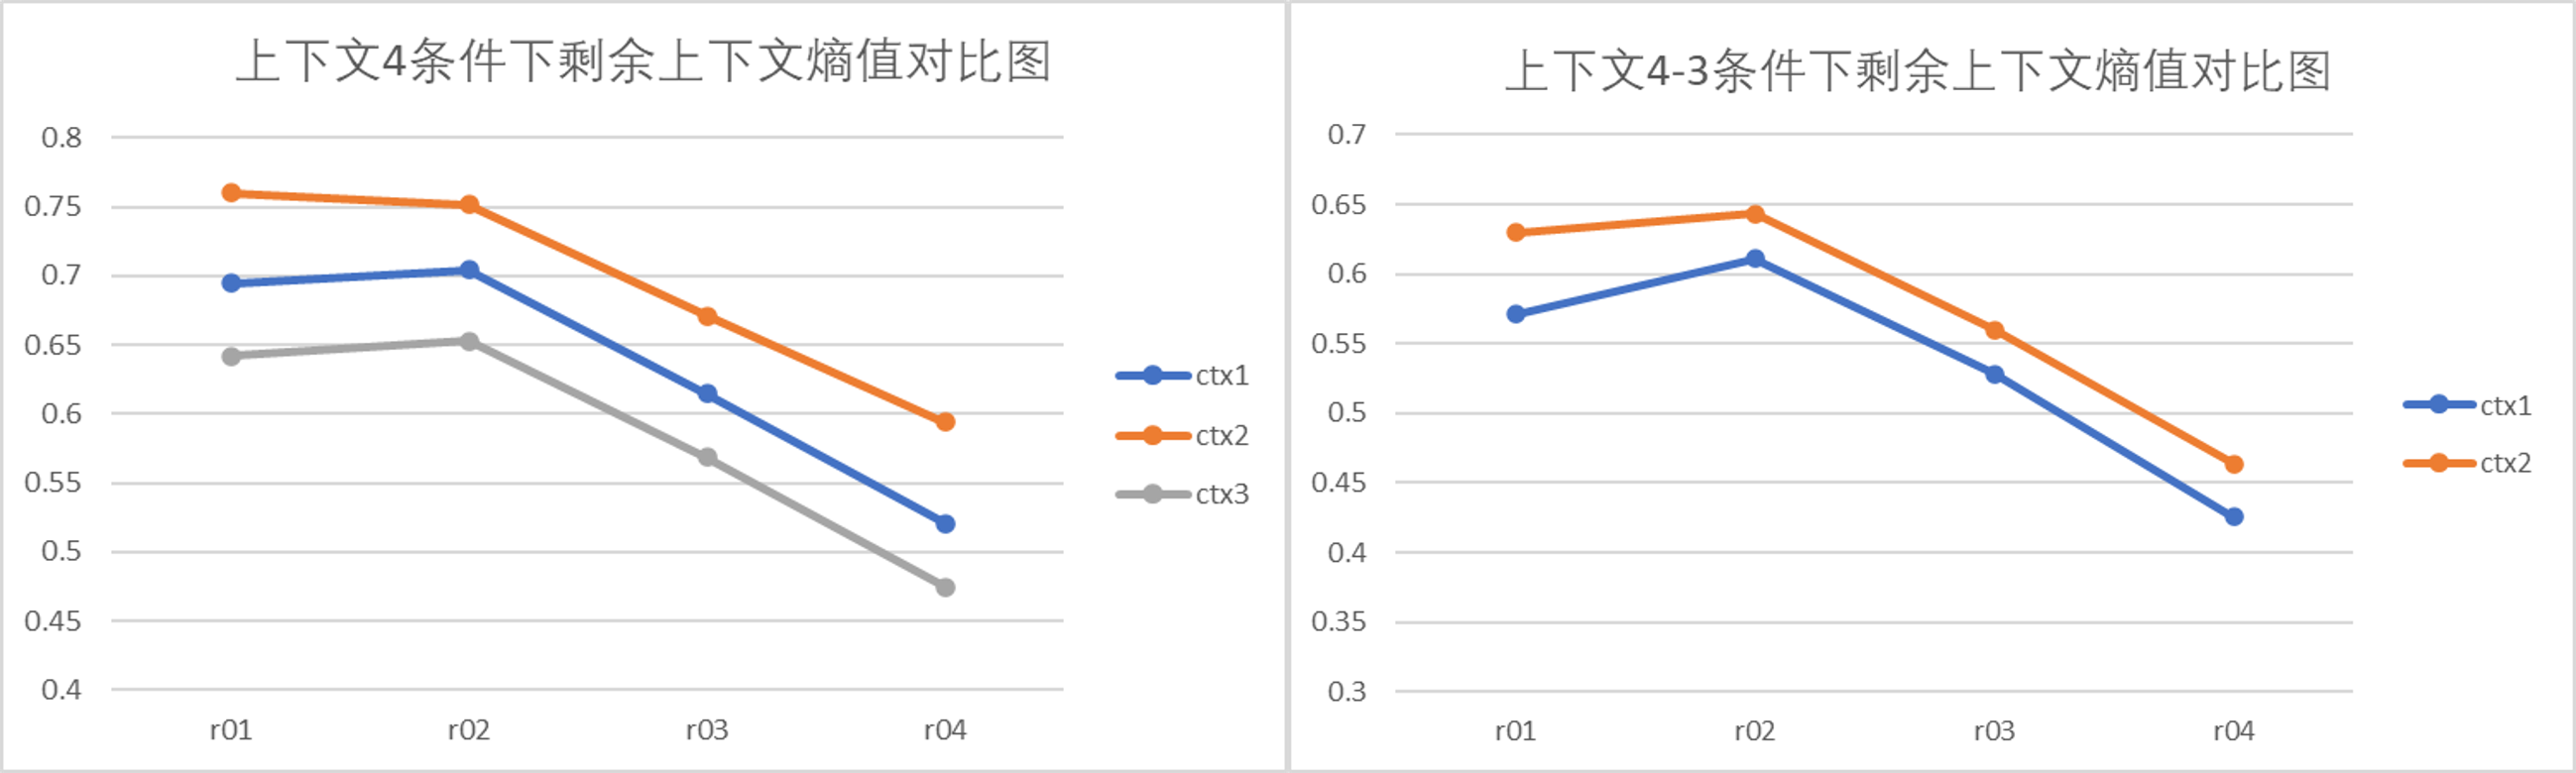
\includegraphics[scale=0.5]{image/高bit位置信息条件熵对比图.png}
    }

    \subfloat[低bit位置信息条件熵对比图]{
        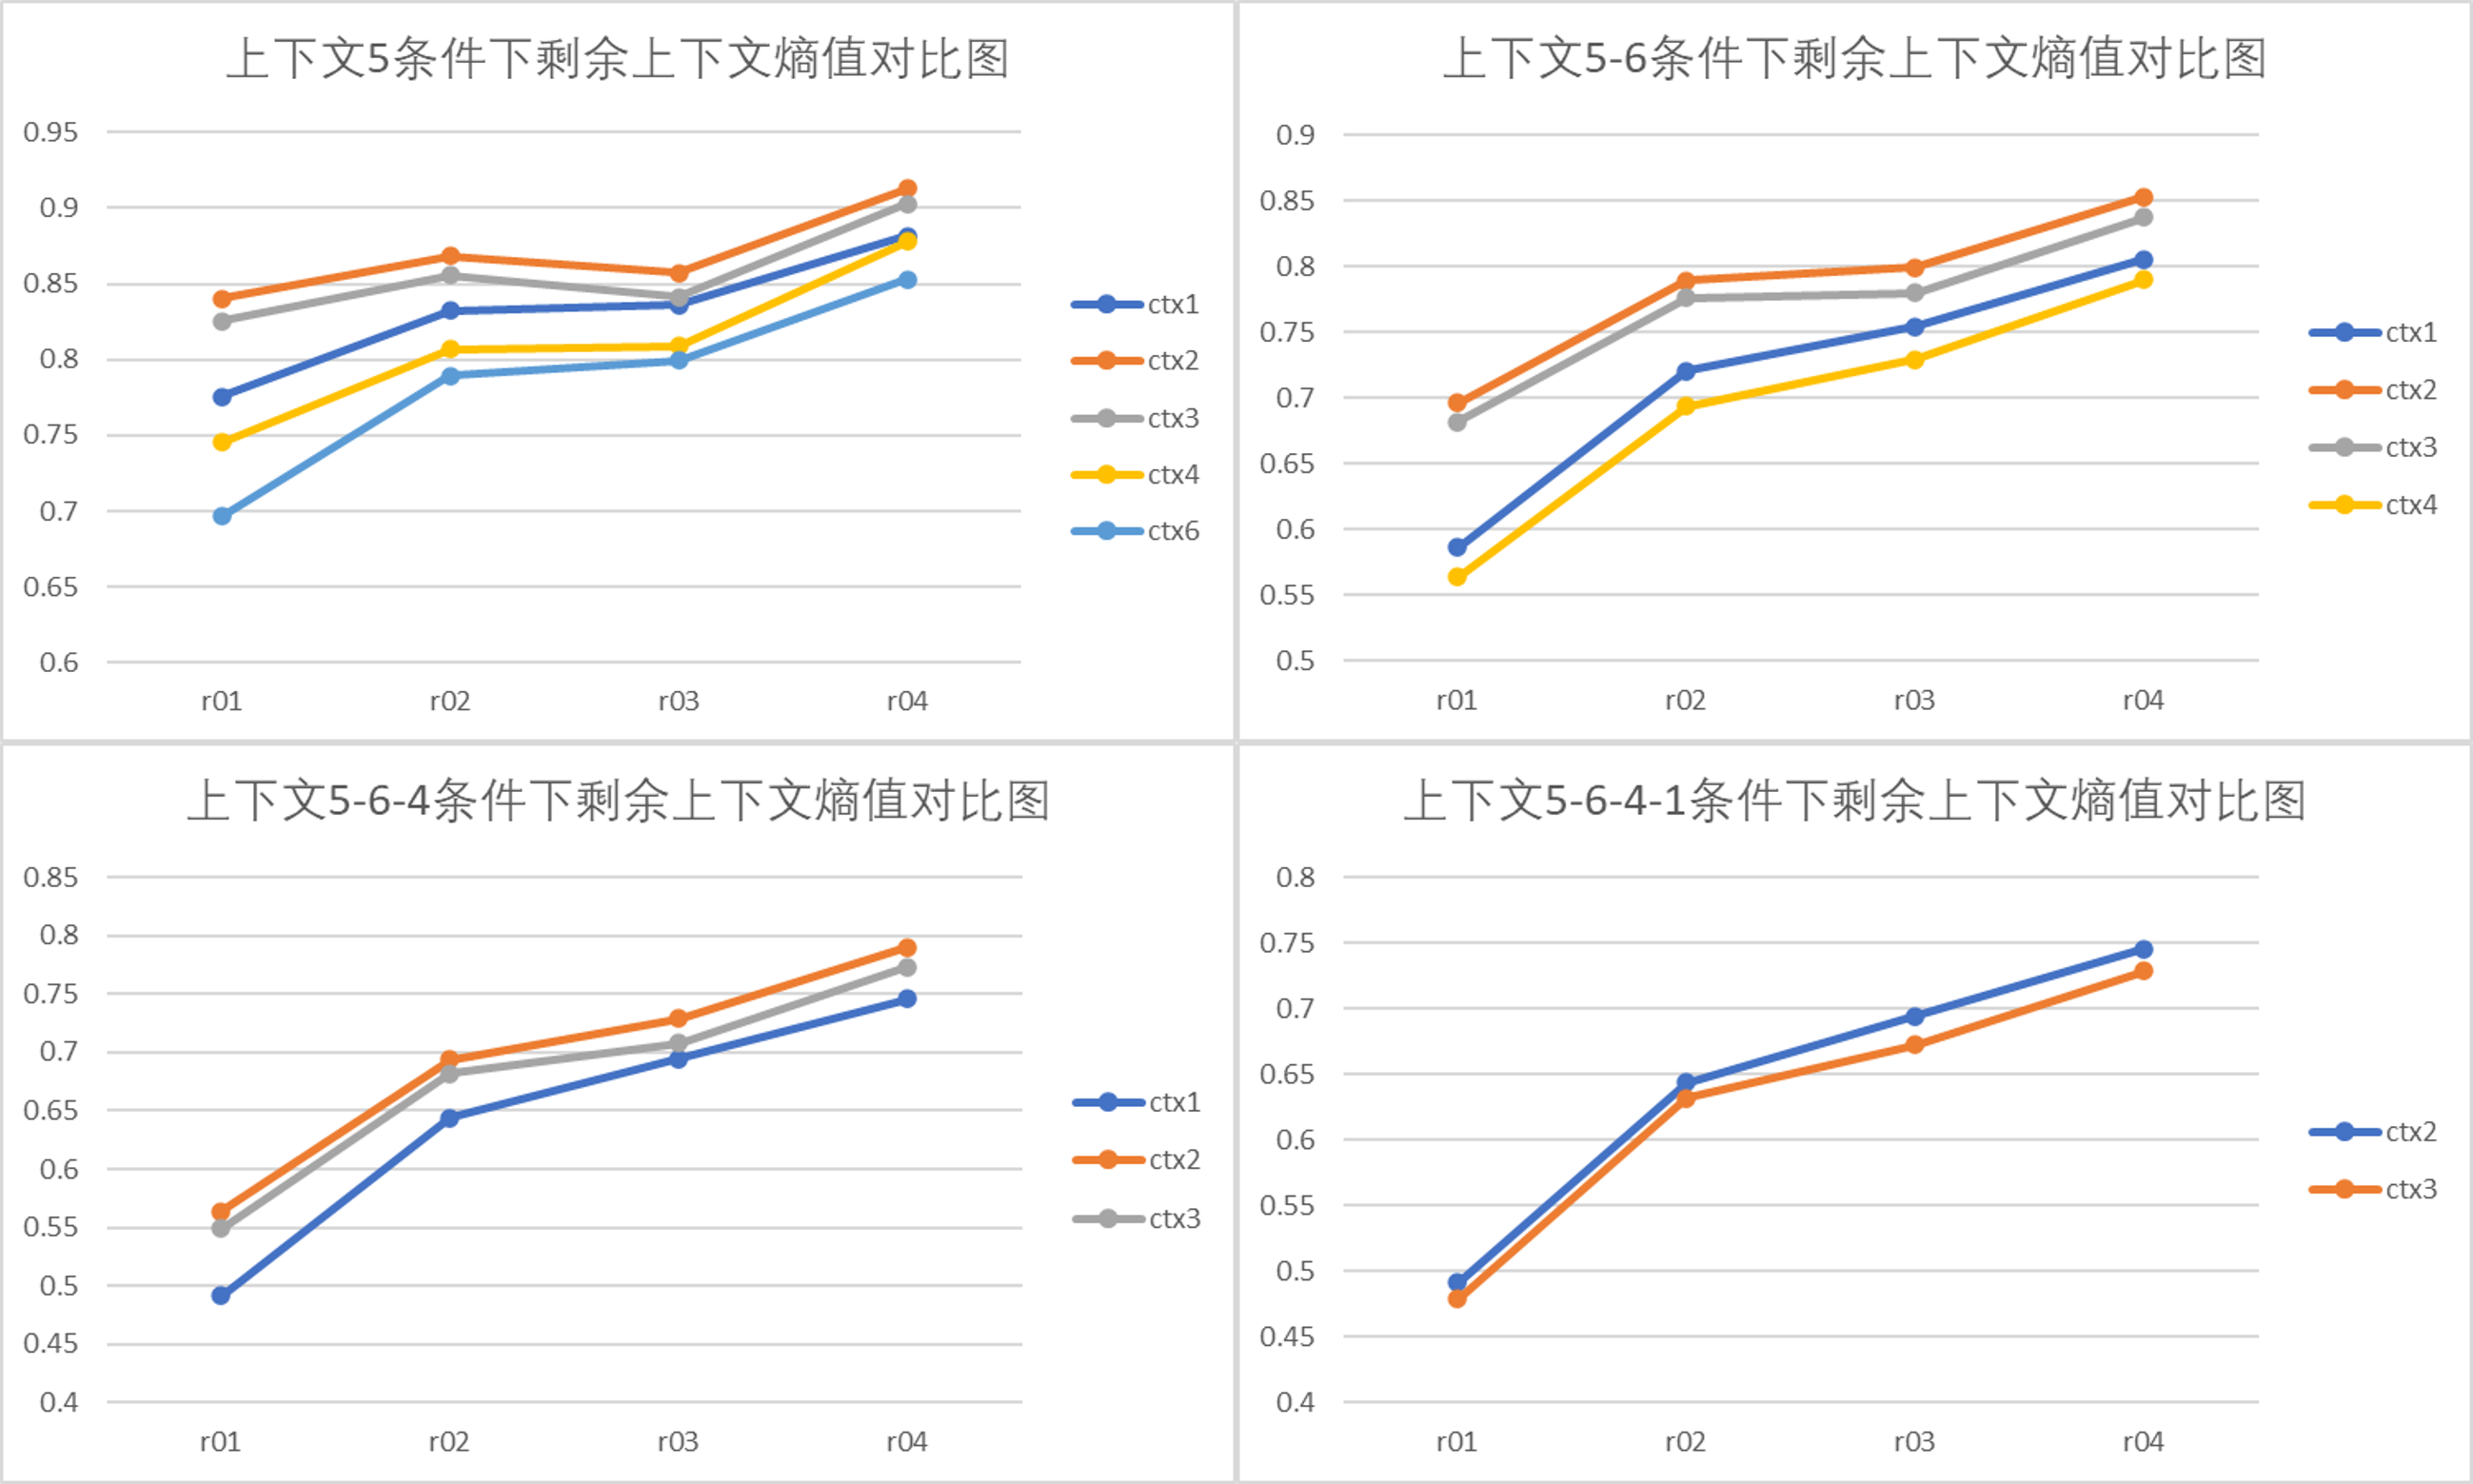
\includegraphics[scale=0.5]{image/低bit位置信息条件熵对比图.png}
    }
    \caption{位置信息条件熵对比图}
    \label{位置信息条件熵对比图}
\end{figure}

由图可以得出,对于编码高bit位置信息时,它所用到的次要信息所包含的上下文的顺序为ctx4-ctx3-ctx1-ctx2;对于编码低bit位置信息时,他所用用到的次要信息所包含的上下文的顺序为ctx5-ctx6-ctx4-ctx1-ctx3-ctx2。
\section{本章小结}
本章首先介绍了Trisoup几何信息编码算法在利用基于OBUF的熵编码时所采用的上下文模型,同时分析了现有上下文模型可能存在的改进空间,然后通过计算并对比各个上下文模型的信息熵与条件熵的大小,得到了一套全新的局部最优的上下文模型。
% \DeclareOption{secret}{\xdu@secrettrue}
% \DeclareOption{english}{\xdu@englishtrue}
% \DeclareOption{print}{\xdu@printtrue}
% \DeclareOption{msfonts}{\xdu@msfontstrue}
% \DeclareOption{adobefonts}{\xdu@msfontsfalse}

\ifx\allfiles\undefined
\end{document}
\fi
%% ----------------------------------------------------------------------
%%% END OF FILE 
%% ----------------------------------------------------------------------